  
\documentclass[t,usenames,dvipsnames]{beamer}
\usetheme{Copenhagen}
\setbeamertemplate{headline}{} % remove toc from headers
\beamertemplatenavigationsymbolsempty

\usepackage{amsmath, tcolorbox, bm, tikz, pgfplots}
\pgfplotsset{compat = 1.16}

\everymath{\displaystyle}

\title{Radical Equations and Inequalities}
\author{}
\date{}

\AtBeginSection[]
{
  \begin{frame}
    \frametitle{Objectives}
    \tableofcontents[currentsection]
  \end{frame}
}

\begin{document}

\begin{frame}
    \maketitle
\end{frame}

\section{Solve radical equations}

\begin{frame}{Solving Radical Equations}
When solving radical equations, we want to try our best to isolate the radical on one side of the equation (if possible). \newline\\	\pause

Then we can raise both sides to the power that is the root of the radical.    \newline\\	\pause

However, sometimes you may end up with extraneous solutions.
\end{frame}

\begin{frame}{Example 1}
Solve each. Remember to check for extraneous solutions.	\newline\\
(a) \quad $\sqrt{5x+1} = 4$
\begin{align*}
\onslide<2->{\sqrt{5x+1} &= 4} \\[6pt]
\onslide<3->{\left(\sqrt{5x+1}\right)^2 &= 4^2} \\[6pt]
\onslide<4->{5x+1 &= 16} \\[6pt]
\onslide<5->{x &= 3}
\end{align*}
\onslide<6->{Check: $\sqrt{5(3)+1} = 4?$}
\onslide<7->{\quad Yes}
\end{frame}

\begin{frame}{Example 1}
(b) \quad $\sqrt{8-x} + 7 = 10$
\begin{align*}
\onslide<2->{\sqrt{8-x} + 7 &= 10} \\[6pt]
\onslide<3->{\sqrt{8-x} &= 3} \\[6pt]
\onslide<4->{8-x &= 9} \\[6pt]
\onslide<5->{x &= -1}
\end{align*}
\onslide<6->{Check: $\sqrt{8-(-1)} + 7 = 10?$}
\onslide<7->{\quad Yes}
\end{frame}

\begin{frame}{Example 1}
(c) \quad $\sqrt[3]{x-10} = 3$
\begin{align*}
\onslide<2->{\sqrt[3]{x-10} &= 3} \\[6pt]
\onslide<3->{\left(\sqrt[3]{x-10}\right)^3 &= 3^3} \\[6pt]
\onslide<4->{x - 10 &= 27} \\[6pt]
\onslide<5->{x &= 37}
\end{align*}
\end{frame}

\begin{frame}{Example 1}
(d) \quad $3\sqrt{x}+12=9$
\begin{align*}
\onslide<2->{3\sqrt{x}+12 &= 9} \\[6pt]
\onslide<3->{3\sqrt{x} &= -3} \\[6pt]
\onslide<4->{\sqrt{x} &= -1} \\[6pt]
\onslide<5->{x &= 1}
\end{align*}
\onslide<6->{Check: $3\sqrt{1}+12=9?$}
\onslide<7->{\quad No}	\newline\\
\onslide<8->{No Solution $\varnothing$}
\end{frame}

\begin{frame}{Example 1}
(e) \quad $\sqrt{2x-7}=\sqrt{3x-12}$
\begin{align*}
\onslide<2->{\sqrt{2x-7} &= \sqrt{3x-12}} \\[6pt]
\onslide<3->{2x - 7 &= 3x - 12} \\[6pt]
\onslide<4->{x &= 5}
\end{align*}
\end{frame}

\begin{frame}{Example 1}
(f) \quad $x-3=\sqrt{x-1}$
\begin{align*}
\onslide<2->{x-3 &= \sqrt{x-1}} \\[6pt]
\onslide<3->{(x-3)^2 &= \left(\sqrt{x-1}\right)^2} \\[6pt]
\onslide<4->{x^2-6x+9 &= x-1} \\[6pt]
\onslide<5->{x^2 - 7x + 10 &= 0} \\[6pt]
\onslide<6->{(x-2)(x-5) &= 0} \\[6pt]
\onslide<7->{x &= 2, 5}
\end{align*}
\end{frame}

\begin{frame}{Example 1 \quad $x-3=\sqrt{x-1}$}
\[x = 2 \quad x=5\]
Check:	\newline\\
\onslide<2->{$x=2$ is extraneous} \newline\\
\onslide<3->{$x=5$ is valid} \newline\\
\onslide<4->{Final answer: $x=5$}
\end{frame}

\section{Solve equations with rational exponents}

\begin{frame}{Equations with Rational Exponents}
When dealing with rational exponents, recall that raising a power to a power will result in multiplying the exponents together. \newline\\	\pause

Using this knowledge, we can isolate the radicand by raising both sides of the equation to the \underline{reciprocal} of the exponent.
\end{frame}

\begin{frame}{Example 2}
Solve each of the following. Remember to check for extraneous solutions.	\newline\\
(a) 	\quad $x^{2/3} = 3$
\begin{align*}
\onslide<2->{x^{2/3} &= 3} \\[8pt]
\onslide<3->{\left(x^{2/3}\right)^{3/2} &= 3^{3/2}} \\[8pt]
\onslide<4->{x &= 3^{3/2}} \\[8pt]
\onslide<5->{&= \sqrt{27}} \\[8pt]
\onslide<6->{&= 3\sqrt{3}}
\end{align*}
\end{frame}

\begin{frame}{Example 2}
(b) 	\quad $\left(x-1\right)^{-2/3} = 1$
\begin{align*}
\onslide<2->{\left(x-1\right)^{-2/3} &= 1} \\[8pt]
\onslide<3->{\left(\left(x-1\right)^{-2/3}\right)^{-3/2} &= 1^{-3/2}} \\[8pt]
\onslide<4->{x-1 &= 1} \\[8pt]
\onslide<5->{x &= 2}
\end{align*}
\end{frame}

\begin{frame}{Example 2}
(c) 	\quad $\left(x+2\right)^{3/2} = -1$
\begin{align*}
\onslide<2->{\left(x+2\right)^{3/2} &= -1} \\[8pt]
\onslide<3->{\left(\left(x+2\right)^{3/2}\right)^{2/3} &= (-1)^{2/3}} \\[8pt]
\onslide<4->{x+2 &= 1} \\[8pt]
\onslide<5->{x &= -1}
\end{align*}
\onslide<6->{\[\text{No solution } \varnothing \]}
\end{frame}

\section{Solve radical inequalities}

\begin{frame}{Solving Radical Inequalities}
When solving inequalities, use the same techniques as solving the equations, then use number lines and test values to solve inequalities.  \newline\\	\pause

This gives us the advantage of solving any inequality after learning how to solve its equation form.	\newline\\	\pause

\alert{\textbf{Important: }} Remember, when dealing with \textbf{even roots}, the domain of the radicand is $\geq 0$.
\end{frame}

\begin{frame}{Example 3}
Solve each of the following and graph your solution on a number line.	\newline\\
(a)	\quad	$\sqrt{x-3} - 3 < 4$
\begin{align*}
\onslide<2->{\sqrt{x-3} - 3 &= 4} \\[6pt]
\onslide<3->{\sqrt{x-3} &= 7} \\[6pt]
\onslide<4->{x-3 &= 49} \\[6pt]
\onslide<5->{x &= 52}
\end{align*}
\end{frame}

\begin{frame}{Example 3	\quad	$\sqrt{x-3} - 3 < 4$}
Critical value of $x$ is 52.	\newline\\
\onslide<2->{For $\sqrt{x-3}$, $x-3$ must be $\geq 0$, so $x \geq 3$}	\newline\\
\onslide<3->{
\begin{center}
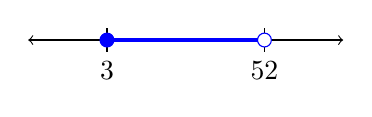
\begin{tikzpicture}
\draw [<->] (-2,0) -- (2,0);
\draw (1,0.15) -- (1,-0.15) node [below] {$52$};
\draw (-1,0.15) -- (-1,-0.15) node [below] {$3$};
\onslide<4->{\draw[color=blue,fill=white] (1,0) circle [radius=2.5pt];
\draw[fill=blue,color=blue] (-1,0) circle [radius=2.5pt];}
\onslide<5->{\draw[color=blue, ultra thick, shorten >= 2.5pt, shorten >= 2.5pt] (-1,0) -- (1,0);}
\end{tikzpicture}
\end{center}
}
\onslide<6->{\[3 \leq x < 52\]}
\end{frame}

\begin{frame}{Example 3}
(b)	\quad	$\sqrt[3]{2x+3} \geq \sqrt[3]{x+12}$
\begin{align*}
\onslide<2->{\sqrt[3]{2x+3} &= \sqrt[3]{x+12}} \\[6pt]
\onslide<3->{2x+3 &= x+12} \\[6pt]
\onslide<4->{x &= 9}
\end{align*}
\onslide<5->{
\begin{center}
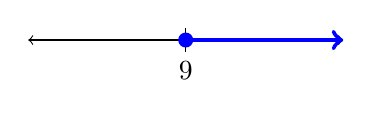
\begin{tikzpicture}
\draw [<->] (-2,0) -- (2,0);
\draw (0,0.15) -- (0,-0.15) node [below] {$9$};
\onslide<6->{\draw[color=blue,fill=blue] (0,0) circle [radius=2.5pt];}
\onslide<7->{\draw[color=blue,ultra thick, ->] (0,0) -- (2,0);}
\end{tikzpicture}
\end{center}
}
\onslide<8->{\[x \geq 9 \]}
\end{frame}

\begin{frame}{Example 3}
(c)	\quad	$\sqrt{2x-1} \leq 2x-1$
\begin{align*}
\onslide<2->{\sqrt{2x-1} &= 2x-1} \\[6pt]
\onslide<3->{\left(\sqrt{2x-1}\right)^2 &= (2x-1)^2} \\[6pt]
\onslide<4->{2x-1 &= 4x^2 - 4x + 1} \\[6pt]
\onslide<5->{4x^2 - 6x + 2 &= 0} \\[6pt]
\onslide<6->{x &= \frac{1}{2}, \quad 1}
\end{align*}
\end{frame}

\begin{frame}{Example 3 \quad $\sqrt{2x-1} \leq 2x-1$}
\begin{center}
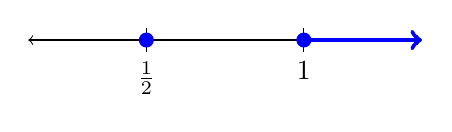
\begin{tikzpicture}
\draw[<->] (-2.5,0) -- (2.5,0);
\draw (-1,0.15) -- (-1,-0.15) node [below] {$\frac{1}{2}$};
\draw (1,0.15) -- (1,-0.15) node [below] {$1$};
\onslide<2->{\draw[color=blue,fill=blue] (-1,0) circle [radius=2.5pt];
					\draw[color=blue,fill=blue] (1,0) circle [radius=2.5pt];
}
\onslide<3->{\draw[color=blue, ultra thick, ->] (1,0) -- (2.5,0);}
\end{tikzpicture}
\end{center}
\onslide<4->{\[x = \frac{1}{2} \quad \text{or} \quad x \geq 1\]}
\end{frame}

\end{document}
